\documentclass[10pt,twocolumn]{article}

\usepackage{geometry}
\geometry{a4paper}
%%\usepackage[cm]{fullpage}

%%\usepackage[top=2in, bottom=1.5in, left=2in, right=1in]{geometry}


\addtolength{\hoffset}{-25pt}
\addtolength{\textwidth}{35pt}


\usepackage{graphicx}
\usepackage{float}
\usepackage{wrapfig}

\linespread{1.} % Line spacing

\graphicspath{{figs/}}

\usepackage{polski}
\usepackage[utf8]{inputenc}

\DeclareFixedFont{\ttb}{T1}{txtt}{bx}{n}{8} % for bold
\DeclareFixedFont{\ttm}{T1}{txtt}{m}{n}{8}  % for normal
\usepackage{color}
\definecolor{deepblue}{rgb}{0,0,0.5}
\definecolor{deepred}{rgb}{0.6,0,0}
\definecolor{deepgreen}{rgb}{0,0.5,0}
\usepackage{listings}


% Python style for highlighting
\newcommand\pythonstyle{\lstset{
language=Python,
basicstyle=\ttm,
otherkeywords={self},             % Add keywords here
keywordstyle=\ttb\color{deepblue},
emph={MyClass,__init__},          % Custom highlighting
emphstyle=\ttb\color{deepred},    % Custom highlighting style
stringstyle=\color{deepgreen},
frame=tb,                         % Any extra options here
showstringspaces=false            %
}}
% Python environment
\lstnewenvironment{python}[1][]
{
\pythonstyle
\lstset{#1}
}
{}
% Python for external files
\newcommand\pythonexternal[2][]{{
\pythonstyle

\lstinputlisting[#1]{#2}}}

\lstset{language=Python}
% Python for inline
\newcommand\pythoninline[1]{{\pythonstyle\lstinline!#1!}}

\title{Rzut ukośny, czyli o prawie Newtona i równaniach różniczkowych}

\begin{document}

\maketitle
\begin{wrapfigure}[10]{l}[0cm]{4cm}
     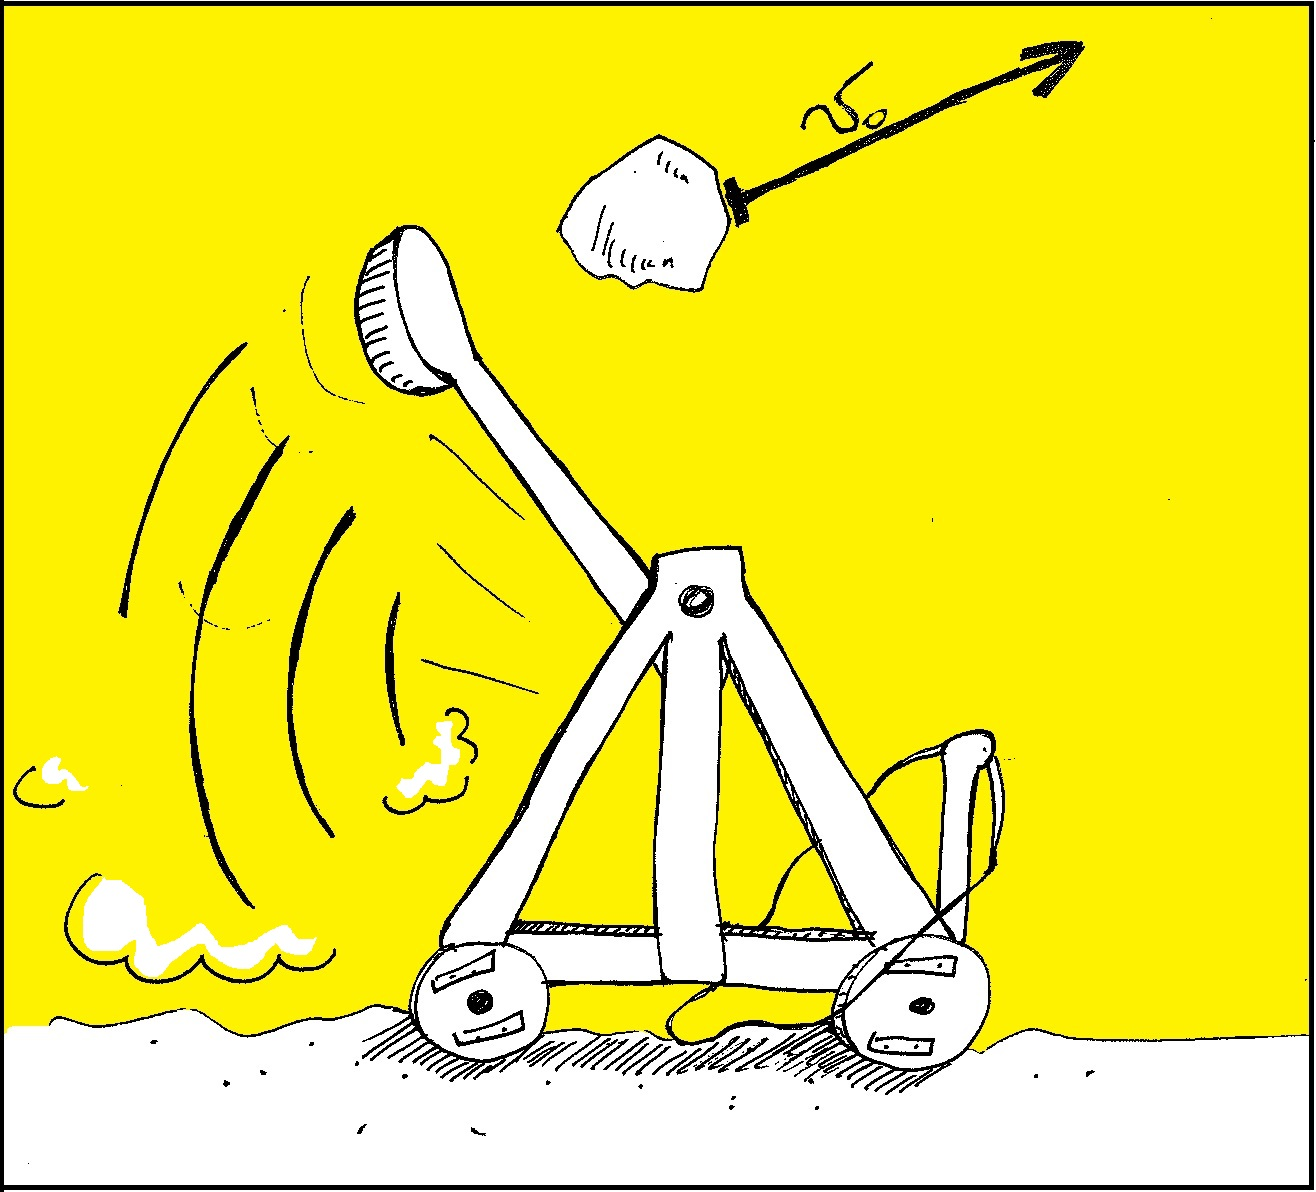
\includegraphics[width=4cm]{3.jpg}
\end{wrapfigure}



Z lekcji fizyki wszyscy wiemy, że prędkość to: $v=\frac{\Delta
  x}{\Delta t}$ a przyspieszenie $a=\frac{\Delta v}{\Delta t}$. Te
pozornie mało spektakularne wzory nabierają Mocy dopiero w zetknięciu
z komputerem. Czytelnika chcącego głębić tajniki metody rozwiązywania
równań różniczkowych, zapraszamy do - aktywnej - lektury tego
artykułu.


Odkrywanie praw fizycznych przez ``komputerowe eksperymentowanie'' z
równaniami jest celem projektu dydaktycznego iCSE prowadzonego na
Uniwersytecie Śląskim. Narzędzie stanowi system Sage\ \cite{sagemath}
będący otwartą implementacją systemu algebry komputerowej z językiem
Python. Sage jest dostępny z poziomu przeglądarceki internetowej
poprzez usługę chmurową\ \cite{cloud} lub serwer pojedynczych obliczeń, na
którym bazuje interaktywna wersja tego artykułu\ \cite{web}.
%
 


\section{Rzut ukośny}

\begin{wrapfigure}[11]{l}[0cm]{5cm}
     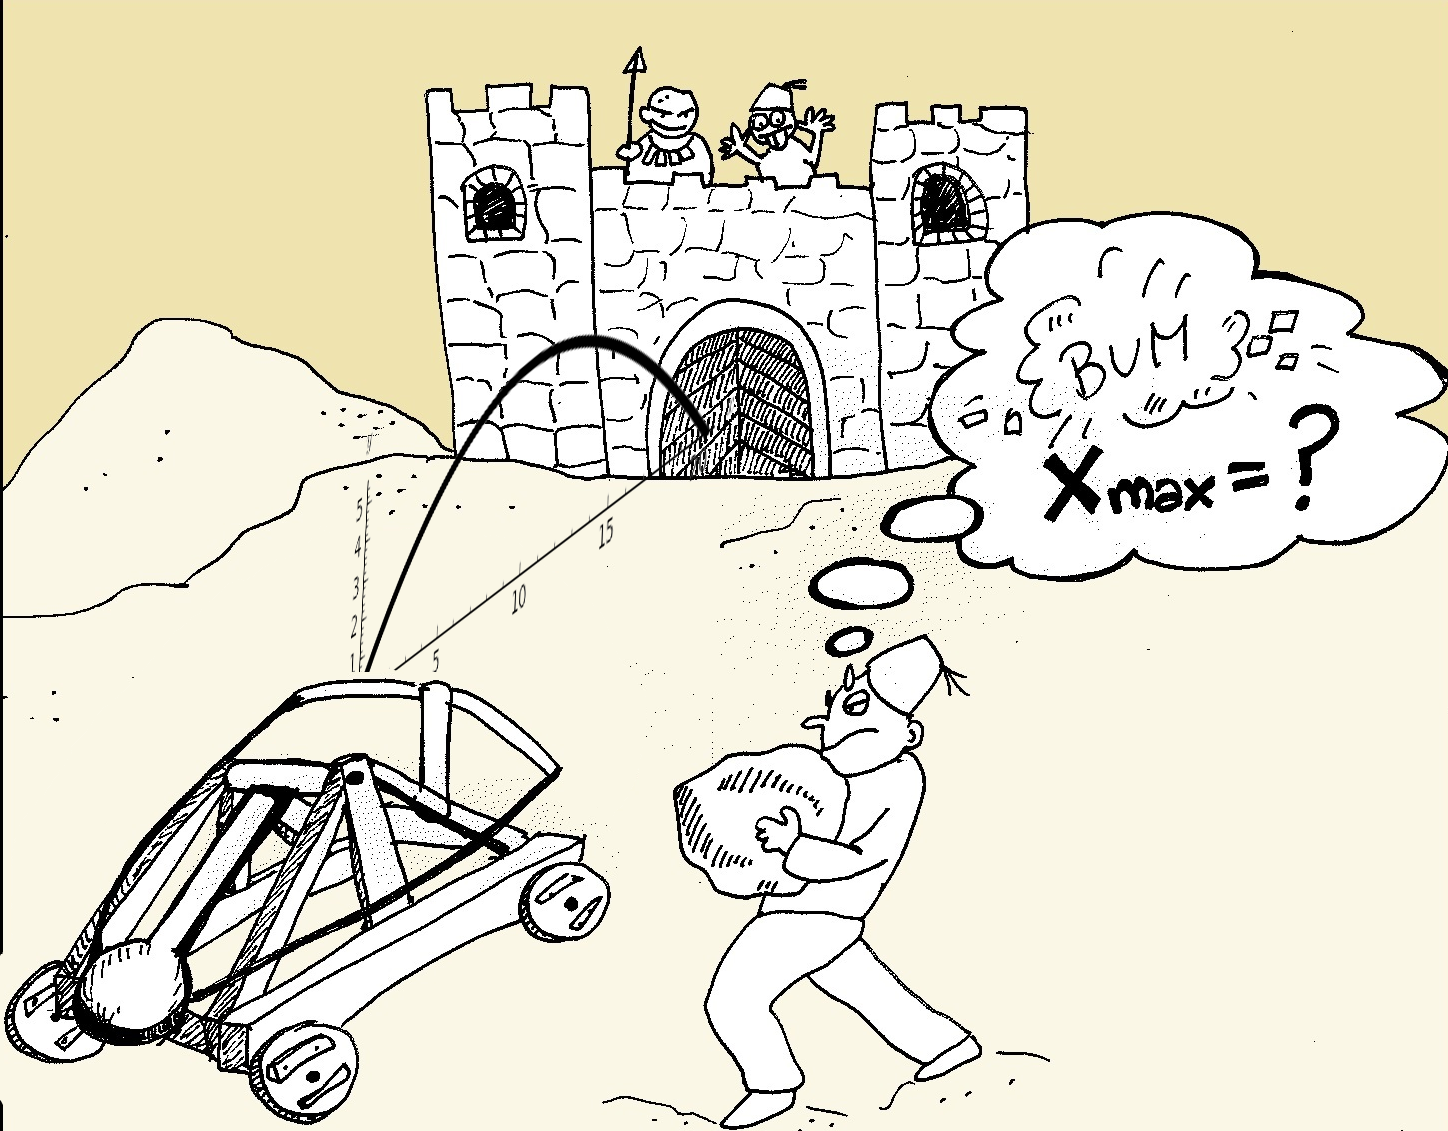
\includegraphics[width=5cm]{1a.png}
\end{wrapfigure}
Rozpoczniemy od pozornie nudnego tematu jakim może się wydawać znany
ze szkoły rzut ukośny. W fizyce, to pojęcie oznacza ruch punktu
materialnego o pewnej masie pod działaniem siły grawitacji. Wiedza na
temat tego zagadnienia była kluczowa podczas konfliktów
zbrojnych. Wysyłając bowiem w stronę wroga punkty materialne w postaci
różnorakich pocisków, chcieliśmy wiedzieć czy aby na pewno dotrą do
celu. Z tego punktu widzenia interesujący jest zasięg posiadanego
przez nas urządzenia miotającego, oczywiście im większy tym
lepszy. Można się spodziewać, że ów zasięg zależy od siły miotającej
naszego urządzenia a co za tym idzie prędkości początkowej
pocisku. Kolejną rzeczą jest uwzględnienie kąta wystrzału. Jeśli
strzelimy pionowo pocisk z pewnością upadnie na nas - zasięg będzie
zerowy. Jeśli strzelimy poziomo to również pocisk nie poleci zbyt
daleko. Pod jakim kątem powinniśmy strzelić?

Odpowiedzi dręczące artylerzystów dostarcza Fizyka, a mówiąc
konkretnie jej gałąź zwana dynamiką. Rozwiązując więc odpowiednie
zagadnienie dynamiki dostajemy tor ruchu tego punktu. 

Podstawowym prawem jest słynna druga zasada dynamiki Newtona, która
wyraża się równaniem:

\begin{equation}
\label{eq:Ni}
m \vec  a = \vec F.
\end{equation}

Podczas lekcji w szkole z reguły rozważa się przypadek, w którym siły
tarcia pomijamy. Wówczas jedyna siła działająca na ciało w ruchu ma to
siła o składowych $(0,-mg)$. Możemy w takim przypadku rozważać ruch
odbywający się w płaszczyźnie rozpiętej przez wektor siły i prędkości
początkowej - czyli nasz pocisk nie będzie skręcał w lewo ani w
prawo. Klasyczne rozwiązanie tego problemu, oparte jest o fakt, że
ruch w pionie $x$ i ruch w poziomie $y$ są od siebie niezależne. W
pionie zachodzi ruch jednostajnie przyśpieszony a w kierunku pionowym
ruch jednostajny. Z lekcji fizyki lub Wikipedii\cite{wikirzut} mamy:
%
\begin{eqnarray}
\label{eq:param}
x(t) &=& x_0+v_{x0} t, \nonumber \\
y(t) &=& y_0 + v_{y0} t - \frac{1}{2}g t^2.
\end{eqnarray}

\noindent Równania (\ref{eq:param}) są tak zwanym parametrycznym
przedstawieniem toru ruchu. Oznacza to, że znamy jak w zależności od
parametru - czasu $t$, zmienia się każda współrzędna. Wyliczając $t$ z
pierwszego i wstawiając do drugiego można łatwo przekształcić te dwa
równania, do postaci funkcyjnej $y=f(x)$. Otrzymamy wtedy równanie
paraboli o ujemnym współczynniku przy drugiej potędze $x$. Jednak w
systemie Sage mamy bardzo wygodną procedurę do rysowania właśnie
takich krzywych parametrycznych - mianowicie funkcję
\verb|parametric_plot|.

\pythonexternal{code01.py}

Rysownie tych krzywych jest tylko fajną zabawą! Wyobraźmy sobie, że
armata ma funkcję działa przeciwlotniczego i pytamy się jakim obszarze
przestrzeni jej pociśki mogą dosięgnąć wrogi samolot?
\begin{wrapfigure}[8]{l}[0cm]{4cm}
     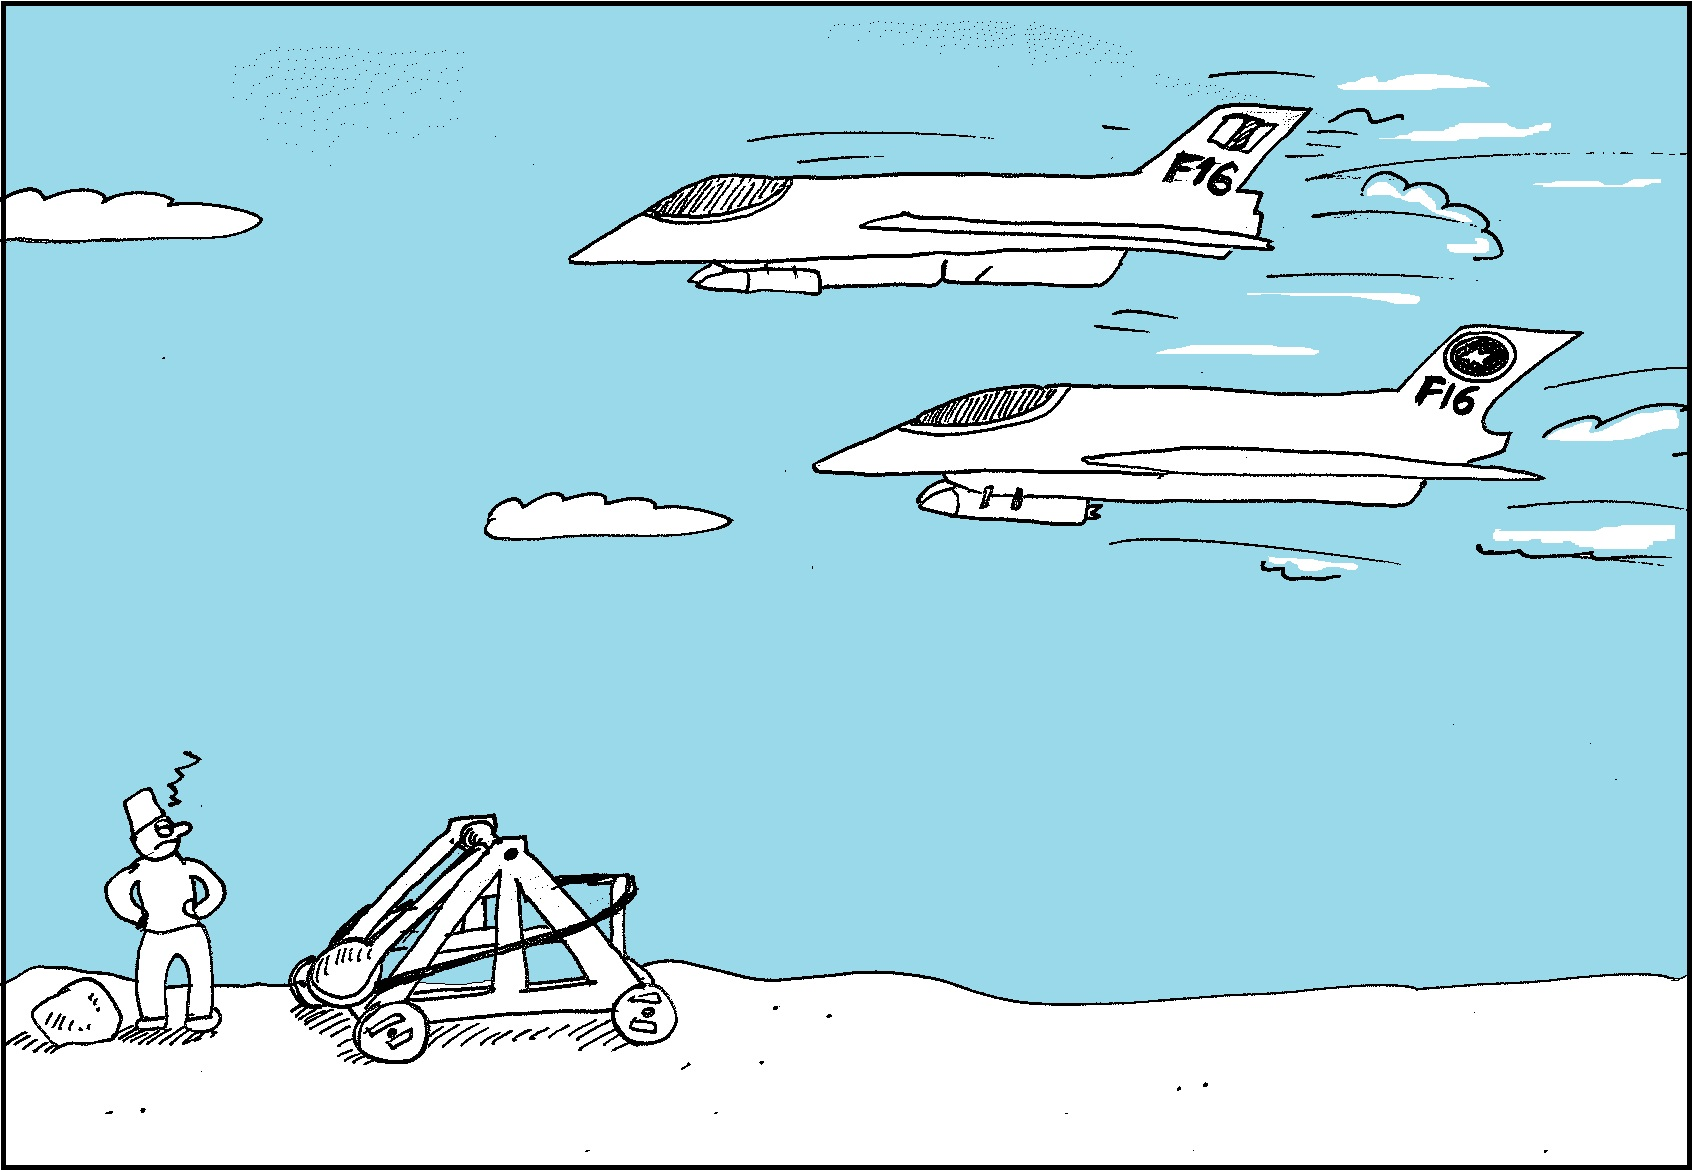
\includegraphics[width=4cm]{2.jpg}
\end{wrapfigure}
Narysujmy w Sage na jednym wykresie tory wystrzałów z prędkościami
$v_{x0}=v_0 \cos(\alpha)$ i $v_{y0}=v_0 \sin(\alpha)$, dla różnych
kątów $\alpha$. Zachęcamy do samodzielnego napisania kodu, który
powinien generować coś zbliżonego do rysunku (\ref{fig:rzut1}).
%
\begin{figure}
    \begin{center}
     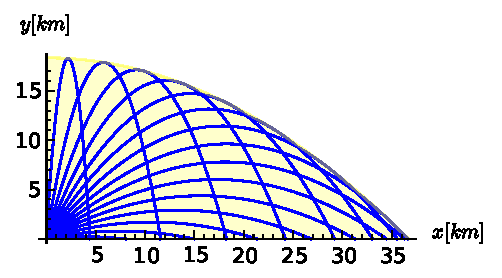
\includegraphics{pplot.pdf}
  \end{center}
  \caption{Obszar rażenia działa o prędkości początkowej pocisku $v_0=600m/s$. 
    \label{fig:rzut1} }
\end{figure}
%
Brzeg obszaru skutecznego ognia działa przeciwlotniczego, jest
matematycznie rzecz biorąc obwiednią rodziny krzywych. Nasz rysunek
sugeruje, że ma on kształt paraboli - i dokładny rachunek pokazuje, że
tak jest rzeczywiście (zob. \cite{web}).


\section{Rzut ukośny - inaczej}

Czytelnik pewnie zastanawia się czy przypadkiem nie chcemy wrobić go w
przerobienie lekcji fizyki pod pretekstem rysowania wykresów funkcji
na komputerze. Otóż nie! Rozwiązanie matematyczne przyda się nam do
weryfikacji wyników rozważań nieco odmiennych niż te prezentowane
zazwyczaj w szkole. Rozważania te umożliwią nam analizę toru lotu
pocisku z uwzględnieniem bardziej realistycznych czynników jak tarcie,
wiatr czy nawet rotacja pocisku. 

W równaniu Newtona dla ruchu pocisku występuje przyśpieszenie. Ze
szkoły wiemy, że jest to zmiana prędkości na jednostkę czasu.
Oznaczmy przez $t$ czas w chwili obecnej a przez $\Delta t$ pewien
mały przyrost czasu. Dla składowej $x$-owej mamy:

\begin{equation}
a_x = \frac{\Delta v_x}{\Delta t}=\frac{v_x(t+\Delta t)-v_x(t)}{\Delta t}. 
\label{eq:dv} 
\end{equation}
%
z prawa Newtona dla składowej $x$-owej mamy:
%
\begin{equation}
a_x = \frac{F_x}{m}
\label{eq:dv} 
\end{equation}
%
więc możemy napisać 
%
\begin{equation}
\frac{v_x(t+\Delta t)-v_x(t)}{\Delta t} = \frac{F_x}{m}.
\label{eq:dv3} 
\end{equation}
 
Załóżmy, że znamy prędkość w chwili $t$: $v_x(t)$ a chcielibyśmy
obliczyć prędkość nieco późniejszej w chwili $t+\Delta t$.  Można by
się pokusić by rozwiązać równanie (\ref{eq:dv3}) na tą prędkości:

\begin{equation}
v_x(t+\Delta t) =v_x(t) + \Delta t\cdot  \frac{F_x}{m}.
\label{eq:euler1} 
\end{equation}
  
Świetnie! Zapiszmy podobne wzory dla drugiej składowej i będziemy
mogli obliczać prędkość w dowolnej chwili czasu. A co z położeniem?
Możemy postąpić podobnie, stosując znany ze szkoły wzór na prędkość,
i tak np. dla $x$:
\begin{equation}
  v_x = \frac{x(t+\Delta t)-x(t)}{\Delta t}
\label{eq:dx}  
\end{equation}
czyli
\begin{equation}
x(t+\Delta t)= x(t)+ \Delta t \cdot v_x 
\label{eq:euler2}
\end{equation}
%
Wzory (\ref{eq:euler1}),(\ref{eq:euler2}) oraz odpowiedniki dla składowych
$y$ układają się w algorytm, który możemy zaprogramować na
komputerze. Ale chwileczkę...

Czy te wzory są poprawne? Niestety nie! W (\ref{eq:euler1}) założyliśmy
prawo dla ruchu jednostajnie przyśpieszonego a siła w ogólności nie
musi być stała, w (\ref{eq:euler2}) założyliśmy, że prędkość jest stała
a nie musi wcale tak być. No chyba, żeby $\Delta t$ było odpowiednio
małe. Wtedy można by się spodziewać, że siła i prędkość w czasie
między $t$ a $t+\Delta t$ nie zmienią się zbyt wiele. Wtedy wzór byłby
przybliżeniem prawdy. Sprawdźmy to eksperymentalnie wykonując poniższy
kod w systemie Sage:

\pythonexternal{code02.py}

\noindent Podobnie jak w przypadku rysowania rozwiązania dokładnego
startujemy z zadania warunków początkowych i parametrów układu (linie
1-3). Następnie zakładamy, że chcemy zastosować przybliżoną procedurę
$m=200$ razy w całego ciągu lotu pocisku. Wyliczamy $\Delta
t=t_{end}/m$ (linia 6). Wykonujemy $m$ razy pętlę w której korzystamy
z czterech przybliżonych wzorów (\ref{eq:euler1}),(\ref{eq:euler2}) i
analogicznych dla komponentu pionowego. Linia 12 jest niezwykle ważna
bowiem ``ustawia'' wyliczone nowe wartości prędkości i położenia jako
warunki początkowe dla kolejnego kroku. W linii 13 dołączamy wybrane
parametry - akurat interesuje nas położenie - do listy punktów
potrzebnych do późniejszego narysowania (dwie ostatnie linie) toru
pocisku. Jeżeli w tej samej sesji Sage wykonaliśmy już pierwszy
program, to możemy łatwo narysować rozwiązanie dokładne i przybliżone
na jednym wykresie komendą: \verb|(p1+p2).show()|.
%
\begin{figure}
    \begin{center}
     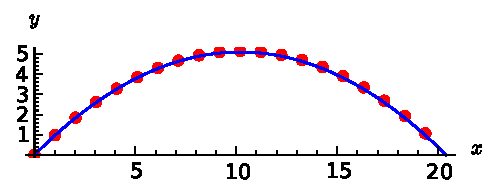
\includegraphics{porownanie.pdf}
  \end{center}
  \caption{Porównanie wyniku dokładnego i metody numerycznej.
    \label{fig:por} }
\end{figure}
%

Na rysunku \ref{fig:por} widzimy, że otrzymaliśmy tor ruchu zbliżony
do dokładnego. Zachęcamy Czytelnika do samodzielnych eksperymentów i
zbadania jak np. ilość iteracji - czyli krok czasowy - wpływa na
wynik. Ciekawostką jest, że nasz program nigdzie nie zawierał funkcji
kwadratowej, a pomimo tego narysował jej wykres - parabolę!
 
Po co robiliśmy tyle szumu i zaprzęgali komputer do obliczania tego co
było z góry tak wiadome?  Przecież w przypadku rzutu ukośnego metoda
numeryczna z mozołem odtwarza wynik analityczny. Okazuje się, że nasz
algorytm może być użyty do rozwiązywania praktycznie KAŻDEGO
zagadnienia opisanego równaniem Newtona! Wystarczy zmodyfikować
siły. Co więcej, siły te mogą zależeć w najdziwniejszy sposób od
każdej ze zmiennych. Wystarczy w naszym algorytmie zmienić zaledwie
dwie linie:

\pythonexternal{code03.py}
% 
\noindent gdzie za $F_x,F_y$ wstawiamy odpowiednie wyrażenia na siły,
które chcemy modelować. Na przykład możemy rozwiązać układ w którym
mamy realistyczną siłę oporu, która zależy kwadratowo od
prędkości. Możemy dodać wiatr i to nawet taki, który wieje inaczej na
100m nad ziemią a inaczej na 10km. Możemy uwzględnić zmianę gęstości
powietrza na dużych wysokościach. W takich przypadkach nie jest łatwo
lub wręcz się nie da otrzymać rozwiązania metodami analitycznymi.

Cierpliwych Czytelników zapraszamy do lektury następnej części tego
artykułu. Niecierpliwych zachęcamy do samodzielnego eksperymentowania
od zaraz.
 
\section{A równania różniczkowe?}

Czyżby dopadła nas cyfrowa demencja - przecież mieliśmy się coś doowiedzieć o
równaniach różniczkowych! 

Okazuje się, że nasz drugi program tak na prawdę był schematem Eulera
rozwiązującym układ czterech równań różniczkowych zwyczajnych!  Skoro
potrafimy już je rozwiązywać, to może dowiedzmy się co to jest?
Mówiąc mniej precyzyjnie, jest to równanie podobne do (\ref{eq:dv3}),
ale w granicy $\Delta t\to0$. Lewa strona przechodzi w wielkość zwaną
pochodną (w tym przypadku pochodną prędkości). Równania różniczkowe to
właśnie takie, które zawierają funkcje (w naszym przypadku
$x(t),v_x(t),y(t),v_y(t),$ i ich pochodne. Przybliżając granicę przez
wzięcie pewnego małego, ale skończonego $\Delta t$ otrzymaliśmy
właśnie schemat numeryczny rozwiązujące nasze równanie różniczkowe.

\begin{thebibliography}{1}

\bibitem{sagemath} http://sagemath.org
\bibitem{cloud} http://cloud.sagemath.com
\bibitem{web} http://visual.icse.us.edu.pl/Warsztaty
\bibitem{wikirzut} http://pl.wikipedia.org/wiki/Rzut\_ukośny

\end{thebibliography}

\end{document}

